\documentclass[
	12pt,				
	openright,		
	twoside,	
	a4paper,
	english,	
	brazil	
	]{abntex2}
\usepackage{lmodern}		
\usepackage[T1]{fontenc}	
\usepackage[utf8]{inputenc}
\usepackage{lastpage}	
\usepackage{indentfirst}
\usepackage{color}	
\usepackage{graphicx}
\usepackage{microtype}

\graphicspath{{./imagens/}}

\usepackage{lipsum}				% para geração de dummy text
\usepackage[brazilian,hyperpageref]{backref}	 
\usepackage[alf]{abntex2cite}	

\renewcommand{\backrefpagesname}{Citado na(s) página(s):~}
\renewcommand{\backref}{}
\renewcommand*{\backrefalt}[4]{
	\ifcase #1 %
		Nenhuma citação no texto.%
	\or
		Citado na página #2.%
	\else
		Citado #1 vezes nas páginas #2.%
	\fi}%

\titulo{Análise de IDPSs}
\autor{Glenon Mateus Barbosa Araújo}
\local{Brasil}
\data{\the\year}
\orientador{Dr. Roberto Samarone dos Santos Araújo}
%\coorientador{}
\instituicao{
  Universidade Federal do Pará -- UFPA
  \par
  Faculdade de Computação
  \par
  Bacharelado em Ciência da Computação}
\tipotrabalho{Trabalho de Conclusão de Curso}
\preambulo{Trabalho de Conclusão de Curso submetida a graduação em Ciência da Computação da UFPA}
\definecolor{blue}{RGB}{41,5,195}
\makeatletter
\hypersetup{
     	%pagebackref=true,
		pdftitle={\@title}, 
		pdfauthor={\@author},
    	pdfsubject={\imprimirpreambulo},
	    pdfcreator={LaTeX with abnTeX2},
		pdfkeywords={abnt}{latex}{abntex}{abntex2}{trabalho acadêmico}, 
		colorlinks=true,       	
    	linkcolor=blue,          
    	citecolor=blue,        	
    	filecolor=magenta,     
		urlcolor=blue,
		bookmarksdepth=4
}
\makeatother
\setlength{\parindent}{1.3cm}
\setlength{\parskip}{0.2cm} 
\makeindex
\begin{document}
\selectlanguage{brazil}
\frenchspacing 

\imprimircapa
\imprimirfolhaderosto*

\begin{fichacatalografica}
	\sffamily
	\vspace*{\fill}
	\begin{center}
	\fbox{\begin{minipage}[c][8cm]{13.5cm}	
	\small
	\imprimirautor
	
	\hspace{0.5cm} \imprimirtitulo  / \imprimirautor. --
	\imprimirlocal, \imprimirdata-
	
	\hspace{0.5cm} \pageref{LastPage} p. : il. (algumas color.) ; 30 cm.\\
	
	\hspace{0.5cm} \imprimirorientadorRotulo~\imprimirorientador\\
	
	\hspace{0.5cm}
	\parbox[t]{\textwidth}{\imprimirtipotrabalho~--~\imprimirinstituicao,
	\imprimirdata.}\\
	
	\hspace{0.5cm}
		1. Suricata.
		2. Snort.
		3. IDPS.
		I. Orientador.
		II. Universidade Federal do Pará.
		III. Faculdade de Computação.
		IV. Análise de IDPSs
	\end{minipage}}
	\end{center}
\end{fichacatalografica}

\begin{errata}
Elemento opcional da \citeonline[4.2.1.2]{NBR14724:2011}. Exemplo:

\vspace{\onelineskip}

FERRIGNO, C. R. A. \textbf{Tratamento de neoplasias ósseas apendiculares com
reimplantação de enxerto ósseo autólogo autoclavado associado ao plasma
rico em plaquetas}: estudo crítico na cirurgia de preservação de membro em
cães. 2011. 128 f. Tese (Livre-Docência) - Faculdade de Medicina Veterinária e
Zootecnia, Universidade de São Paulo, São Paulo, 2011.

\begin{table}[htb]
\center
\footnotesize
\begin{tabular}{|p{1.4cm}|p{1cm}|p{3cm}|p{3cm}|}
  \hline
   \textbf{Folha} & \textbf{Linha}  & \textbf{Onde se lê}  & \textbf{Leia-se}  \\
    \hline
    1 & 10 & auto-conclavo & autoconclavo\\
   \hline
\end{tabular}
\end{table}

\end{errata}

\begin{folhadeaprovacao}

  \begin{center}
    {\ABNTEXchapterfont\large\imprimirautor}

    \vspace*{\fill}\vspace*{\fill}
    \begin{center}
      \ABNTEXchapterfont\bfseries\Large\imprimirtitulo
    \end{center}
    \vspace*{\fill}
    
    \hspace{.45\textwidth}
    \begin{minipage}{.5\textwidth}
        \imprimirpreambulo
    \end{minipage}%
    \vspace*{\fill}
   \end{center}
        
   Trabalho aprovado. \imprimirlocal, 24 de novembro de 2012:

   \assinatura{\textbf{\imprimirorientador} \\ Orientador} 
   %\assinatura{\textbf{Professor} \\ Convidado 1}
   %\assinatura{\textbf{Professor} \\ Convidado 2}
   %\assinatura{\textbf{Professor} \\ Convidado 3}
   %\assinatura{\textbf{Professor} \\ Convidado 4}
      
   \begin{center}
    \vspace*{0.5cm}
    {\large\imprimirlocal}
    \par
    {\large\imprimirdata}
    \vspace*{1cm}
  \end{center}
  
\end{folhadeaprovacao}
\begin{dedicatoria}
   \vspace*{\fill}
   \centering
   \noindent
   \textit{•} \vspace*{\fill}
\end{dedicatoria}
\begin{agradecimentos}

\end{agradecimentos}
\begin{epigrafe}
    \vspace*{\fill}
	\begin{flushright}
		\textit{•}
	\end{flushright}
\end{epigrafe}
\setlength{\absparsep}{18pt} % ajusta o espaçamento dos parágrafos do resumo
\begin{resumo}

 \textbf{Palavras-chave}: Segurança, Suricata, Snort, Sistema de Detecção de Intrusão, Sistema de Prevenção de Intrusão, IDS, IPS.
\end{resumo}

\begin{resumo}[Abstract]
 \begin{otherlanguage*}{english}

   \vspace{\onelineskip}
 
   \noindent 
   \textbf{Keywords}: Security, Suricata, Snort, Intrusion Detection System, Intrusion Prevention System, IDS, IPS.
 \end{otherlanguage*}
\end{resumo}

\pdfbookmark[0]{\listfigurename}{lof}
\listoffigures*
\cleardoublepage
\pdfbookmark[0]{\listtablename}{lot}
\listoftables*
\cleardoublepage
\begin{siglas}
  \item[IDS] \textit{Intrusion Detection System}
  \item[IPS] \textit{Intrusion Prevention System}
\end{siglas}
\pdfbookmark[0]{\contentsname}{toc}
\tableofcontents*
\cleardoublepage
\textual
\chapter*[Introdução]{Introdução}
\addcontentsline{toc}{chapter}{Introdução}
\section*{Objetivos}
\section*{Trabalhos Relacionados}
\section*{Motivação}
\chapter{Segurança de Redes de Computadores}
\section{Cenário Geral}
\section{Ataques}
\subsection{Varredura de Redes}
\subsection{Exploração de Vulnerabilidades}
\subsection{Força Bruta}
\subsection{Desfiguração de páginas}
\subsection{Negação de Serviços}
\subsection{Worm}
\subsection{Trojan}
\subsection{Fraudes - Direitos Autorais}
\chapter{Sistemas de Detecção e Prevenção de Intrusão}
\section{Tipos de IDS/IPS}
\section{Snort}
\section{Suricata}
\chapter{Detecção de Intrusão em um Cenário Real}
%- Em cada capitulo adicionar um texto introdutório
%- Adicionar o seguinte texto:
Este capítulo esta organizado da seguinte forma: A próxima seção apresenta o cenário de testes, que fala das caracter
%Este capítulo esta organizado da seguinte forma: A proxima seção
%aprensenta .... A Seção XY apresenta...
\section{Cenário de Testes}
%Descrever o cenário. Ex: Uma rede com XXX usuários; Os usuários utilizam
%diferentes ferramentas,...
%Adicionar gráficos de utilização da rede
A rede selecionada para ser monitorada tem os valores especificados na tabela \ref{tabela-tráfego}. Podemos verificar que seu pico de trafego chega a 107,25 Mbps em um determinado período do dia, valores considerados ideais para o experimento, inclusive para tentar validar os recursos alocados.

\begin{table}
 \centering
 \begin{tabular}{|c|c|c|c|c|}
 \hline
  & último & min & méd & máx \\
 \hline
 média & 29,34 Mbps & 0 bps & 5,45 Mbps & 107,25 Mbps \\
 \hline
 \end{tabular}
 \caption{Estatística do trafego da rede selecionada para teste}
 \label{tabela-tráfego}
\end{table}
\section{Infraestrutura definida para testes}
%Descrever o que foi utilizado:
%Ex: Equipamentos - Servidores, ....
%    Configuração
%    Ferramentas - Snort (referenciar capítulo), ...
No ambiente de teste foi usado uma máquina Dell com 134G de memória RAM e 40 núcleos. Usou-se XenServer \cite{xenserver} versão 7, sistema operacional (SO) \textit{opensource} da Citrix voltado para virtualização. Foram testados outros SOs porém somente o XenServer possuía, na época da instalação do ambiente, \textit{firmware} da placa de rede do \textit{host} compatível e que funcionava com instabilidade. Outro fator que pesou na escolha do SO foi a experiência que tinha com a plataforma.

No primeiro momento, foi instalado uma máquina virtual que seria usada como base para instalações de outras máquinas usando o recurso de \textit{snapshot} do sistema. O uso desse recurso foi necessário para criar um ambiente igual para os IDSs.

Foi alocado 8 GB de memória RAM, 4 processadores e 100 GB de espaço em disco para o \textit{snapshot}. Esses valores foram definidos com base em um estudo \cite{mikelococo} que considerava vários fatos, como largura da rede, localização do IDS e versão e tipo do capturador de tráfego para dimensionar os recursos, aplicado especificamente ao Snort. A mesma regra foi aplicada ao Suricata.

Para o \textit{host} conseguir pegar o pacotes destinados a rede selecionada foi necessário uma configuração de espelhamento que consiste na copia dos pacotes que saem pela porta dessa rede no \textit{switch} para a porta conectada no \textit{host}. A interface de rede do \textit{host} precisou ser configurado no modo promisc.

Posteriormente criou-se três máquinas virtuais, duas usadas para instalação dos IDSs (Suricata e Snort) e a terceira para instalação das ferramentas usadas para simular ataques a rede. Optou-se pela instalação do sistema Kali \cite{kalilinux} para geração de ataques pois nele existe várias ferramentas nativas para testes de penetração e auditoria de segurança.
 
Para coleta das informações de uso de recurso de hardware como memória, processamento e I/O das máquinas com os IDSs foi usado o \textit{daemon} Collectd \cite{collectd}. Outra opção para esse fim é a utilização de um servidor de monitoramento com o \textit{Zabbix} \cite{zabbix}. A ideia de usar duas ferramentas para analise é fazer um comparativo e validar as informações coletadas.

\begin{figure}
 \centering
 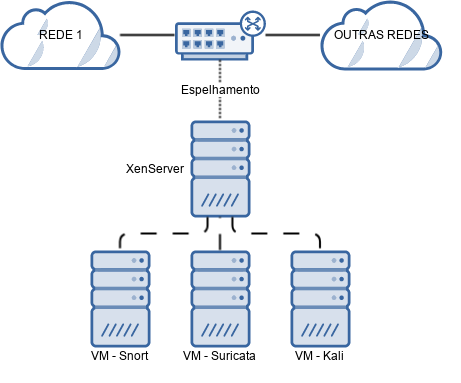
\includegraphics[scale=.7]{infra.png}
 \caption{Infraestrutura do ambiente de teste}
 \label{infra-ambiente}
\end{figure}
\section{Testes Realizados}
%Quais os testes realizados com justificativa ?
%Descrição dos testes. Quais os testes foram realizados ?
\section{Resultados}
%Resultados esperados e obtidos
%Quais os resultados dos testes ??
%Comparação das ferramentas
%Problemas encontrados
\section{Conclusão}
\section{Métricas de Comparação}
%Consumo dos Recursos de Hardware (Memória, Processamento)
%Taxa de Detecção
%Número de Falsos Positivos/Negativos
% ----------------------------------------------------------
\chapter{Considerações Finais}
\phantompart
\postextual
\bibliography{dissertacao}
\phantompart
\printindex
\end{document}
